\startfirstchapter{Introduction}
\label{chapter:introduction}
The vulnerability of the software enable the exploitation of the computer or system it is running on. Wherefore, the emphasize placed on computer security particularly in the field of software vulnerabilities increase dramatically along with the grow of the internet. It's important for software developers to build secure applications. Assurance about the integrity and security of the software are expected from the vendors of the software. Unfortunately, building secure software is expensive. The vendors usually comply with their own quality assurance measures which focus on marketable concerns while left security in lower priority or even worse, totally ignore it. Therefore, fully relying on the vendor of the software to secure your system and data is unpractical and risky.

Software security review conducted by a third party is usually more convincing and reliable. One approach of software security review is software auditing. It is a process of analyzing the software in forms of source code or binary. This auditing can uncover some hard to reveal vulnerabilities which might be exploited by the hackers. Identification of these security holes can save the users of the software from putting their sensitive data and business resources at risk.

Most of the software vulnerabilities are caused by malicious data intrusion. So it is valuable to understand how this malicious data trigger the unexpected behaviors of the system. In most of the cases, this malicious data is injected by attackers into the system to trigger the exploitation. Nonetheless, this malicious data might go through devious path to ultimately trigger an exploitable condition of the system. In some complicated system, several components which are collaborated programs work together to provide service or functionality. In these situation, the malicious data might have passed through multiple components of the system and be modified before it reach the vulnerable point of the system. As a consequence, the flow of data throughout the system's different programs is considered to be one of the most important attribute to analysis during the security review.\cite{dowd_art_2006}

The data flow among various programs with in the system or across different systems helps to understand how the system work as well as disclose the vulnerabilities of the system as stated before. There are multiple mechanism to grab the data across programs. And the methods for obtaining this data flow is essential and can affect the analysis result greatly. 

In this research, I developed a method to analysis communications between the programs by the analysis of the execution traces of them. I didn't aim at covering all the communication types but only focus on the data exchanging ones. This method can guide the security engineers to investigate the communications of the programs in the circumstance that they have the captured execution traces and want to understand the interaction behavior of the programs. The research is not specified for vulnerabilities detection but generalized for the comprehension of the behavior of the programs.

\section{Motivation}
This project started with an informal requirement from DRDC for visualizing multiple assembly traces to assist their software and security analysis. The literature review and the conversation with DRDC help to clarify the goal and target of this research. In this section, I discuss the need of performing assembly trace investigation for communication analysis. First I explain why the security engineers perform assembly trace analysis. Then I elaborate why they need to perform communication analysis at assembly trace level. 

\subsection{Why Assembly Trace Analysis}
Dynamic analysis of program is adopted mainly in software maintenance and security auditing\cite{zhang2010detecting}, \cite{cai2016sworddta}, \cite{somorovsky2016systematic}. Sanjay Bhansali et al. claimed that program execution traces with the most intimate detail of a program's dynamic behavior can facilitate the program optimization and failure diagnosis. Jonas Tr{\"u}mper et al. give a example of how tracing can facilitate software-maintenance tasks \cite{trumper2012maintenance}.

The dynamic analysis can be done by using debuggers, however, debuggers would halt the execution of the system and result in a distortion of the timing behavior of the running system \cite{trumper2012maintenance}. Instead, tracing a running program with instrumentation would provide more accurate run time behavior information about the system.

The instrumentation of the tracing can be in various levels, such as programming language or machine language levels. The choice in some how depends on the accessibility to the application. The application access is divided into five categories with variations: source only, binary only, both source and binary access, checked build, strict black box. Binary only category is common when performing vulnerability research on closed-source commercial software.\cite{dowd_art_2006} In this case, assembly level tracing provides the possibility of the security review of the software.

On the other hand, since the binary code is what is running on the system, it is more representative of actual situation than the source code.  Some bugs might appear because of a compilation problem or because the compiler optimized away some code that was
necessary to make the system secure. A piece of code listed below is an example in which the line of code resetting the password before the program end would be optimized away by GNU Compiler Collection(GCC) due to it is not used later. This made the user's password stayed in memory, which is considered as a security flaw. However, by looking at the source code didn't reveal that problem.

\begin{lstlisting}[language=C++, caption= Password Fetching Example ]
#include <iostream>
#include <string>
#include <conio.h>
using namespace std;
int main(){
   string password ="";
   char ch;
   cout << "Enter password";
   ch = _getch();
   while(ch != 13){//character 13 is enter
      password.push_back(ch);
      cout << '*';
      ch = _getch();
   }   
   if(checkPass(password)){
     allowLogin();
   }  
   password ="";
}
\end{lstlisting}

\subsection{Why Communication Analysis with Assembly Traces}
Programs nowadays do not alway work isolated,  many software  appear as  reticula collaborating systems connecting different modules in the network\cite{PhysRevE.68.046116} which make the discovery of vulnerabilities even harder. The communication and interaction between modules affect the behavior of the software. Without regarding to the synergy information, analysis of the isolated execution trace on a single computer is usually futile. The tracing data flow process is essential to reviews of both the design and implementation of software.

Many network sniffer such as Wireshark\cite{_wireshark_????} and Tcpdump\cite{tcpdump_tcpdump/libpcap_????} can help to capture the data flow across the network which make the systematic analysis possible. However, it is claimed as the insufficient method due to the fact that security problems can occur even if the information sent is correct. Therefore, analyzing the communications with transmitted data in instruction and memory access level is a solid way to evaluation the system.

Shameng Wen et al. argued that fuzz testing and symbolic execution are widely applied to detect vulnerabilities in network protocol implementations. They present their model-guided approach to detect vulnerabilities in the network protocol implementation. Their work focus on designing the model which guide the symbolic execution for the fuzz testing but ignoring the analysis of the output, which is the execution traces. \cite{wen2017model} Further more, their work focus only on the network protocol implementation but not generalized to all communications, including network protocol and inter process communications.

Besides vulnerabilities detection and security reason, communication analysis with assembly traces can also be a way to learn how the work is performed by the system or sometime validate a specification of it. Our research partner DRDC provided some use cases in which they require the assistance of communication analysis to understand their systems. The first one is related to their work with the embedded systems. These systems often have more than one processor, each specialized for a specific task, that coordinate to complete the overall job of that device.  In the other case, the embedded device will work with a normal computer and exchange information with it through some means
(USB, wireless, etc.).  For instance, the data might be coming in from an external sensor in an analog form, transformed by a Digital Signal Processor (DSP) in a device, sent to a more generic processor inside that device to integrate with other data then send wireless to an external computer. Being able to visualize more than one trace would help them follow the flow of data through the system.

\section{Research Goal}
The goal of this research is to design a method for communication analysis using the execution traces of the interacting programs. This method should be general enough for all message based communication analysis between programs regardless of their programming language, host operating system or selected execution tracer. 

\section{Research Process}
Figure \ref{methodology} shows the overview of my research process with three abstracted stages. However, The approach of this research is not a forthright process. Instead, it is a back and forth one, for example the implementation changed several times with the changes of the model, and the models was modified based on the understanding throughout the implementation. 

\begin{figure}[H]
  \centerline{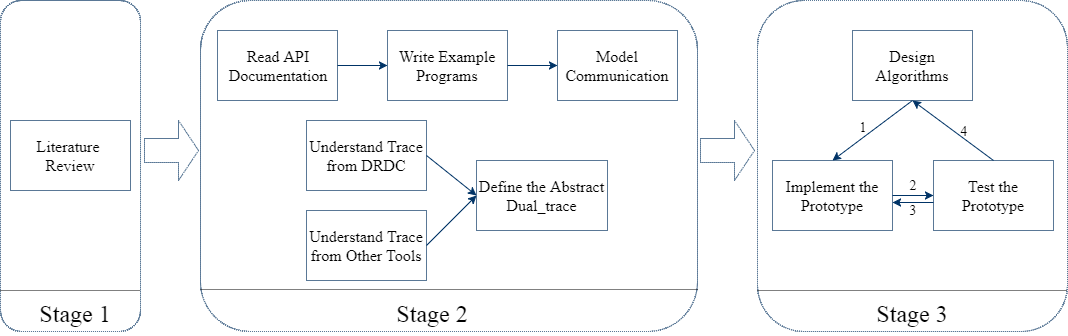
\includegraphics[scale=0.45]{Figures/methodology}}
  \caption{Research Approach overview}
  \label{methodology}
  \end{figure}

This research requires background knowledge in three major fields: 1)software security, 2)program communication mechanisms and implementations, 3)program trace in assembly level. I acquired the background knowledge basically from literature review. It helps me to grab the essential concept of software vulnerabilities and their categories, understand some facilities for vulnerabilities detection and software maintenance in the perspective of security. After that, I was convinced that communication analysis in assembly trace level would benefit software security engineers to understand to behavior of the software and detect software vulnerabilities. 

In order to analysis the communication of programs, I had to know how the communication works. For this purpose, I started the investigation from a piratical experiment by writing example simple programs with the Windows API and run them locally in my desktop. By understanding their behavior and the reading of the Windows API documentation, I abstracted the communication model which is not operating system specified.

The abstract assembly trace definition was build on the generalization of the trace format provided by our research partner, DRDC. I don't have the access to their home-made assembly tracer which is based on PIN\cite{_pin_????}. Fortunately, they provides a comprehensive document about the format of the captured trace and example traces to me. With these, I grasped the constructive view of the assembly execution trace. Further more, in the present of some dynamic software analysis works \cite{godefroid2008automated}, \cite{li2013software}, \cite{sailer2016coretana}, \cite{balakrishnan2004analyzing}, \cite{bhansali2006framework} and \cite{trumper2012maintenance}, it is certain that, some other tools can also capture the required information in assembly level for communication analysis. This supports the generalization of the trace definition and the abstraction of the dual\_trace.

The implementation of the prototype and the communication analysis algorithms are develop in parallel. The high level communication identification algorithm and the specific algorithms for named pipe communication methods were abstracted based on the implementation, while the others are developed theoretically. Two experiments are designed to test the prototype and some algorithms. 


\section{Contribution}
The main contributions of these work can be summarized as:
\begin{itemize}
  \item \textbf{Communication Model:} The communication model in this thesis is an abstract model of the communications between two programs. It was abstracted from the understanding of several communication methods and is general for other communication methods that are not mention in this thesis.
  \item \textbf{Dual\_trace Formalization:} By understanding the assembly level execution traces, a dual\_trace was formalized to describe the information that needed for communication analysis. This model doesn't specify the format of the execution traces but defines what information is necessary to be contained to fulfil the analysis requirement. All execution traces comply with this definition can be used for the analysis.
  \item \textbf{Communication Analysis Approach:} The overall approach to identify the communication of a communication method is designed. Some algorithms are developed for the steps in this approach regarding to some communication methods or communication categories.
  \item \textbf{Feature Prototype:} A prototype is designed and implemented on Atlantis. This prototype prove the communication analysis approach is feasible. It is a unique tool for the security engineers to analysis the communications of programs via assembly execution trace analysis.
\end{itemize}

\section{Thesis Organization}
In Chapter 2, I summarize the related background information and knowledge needed to understand or related to this work including security and vulnerability, program communication mechanisms, program execution trace tools, and Atlantis. 

Chapter 3 depicts the model of the communication between two programs. The communication model defines the communication in the context of trace analysis as well as discusses the properties of the communications. 

Chapter 4 presents the abstract dual\_trace definition. Based on this definition, I developed the communication analysis process and the essential algorithms.

To provide more concrete idea, I present, in chapter 5, the implemented dual\_trace communication analysis prototype. This prototype was built on top of Atlantis\cite{huang2017atlantis}, an assembly execution trace analysis environment.

In chapter 6, I present two experiments of communication analysis with dual\_traces of programs using the implemented prototype. Notably, the result shows the communications are correctly identified. 

Finally, In chapter 7, I conclude the result of this research and outline the possible future work.